\title{[Lab8] Deep Q-Network and Deep Deterministic Policy Gradient}
\author{0616014 楊政道}
\maketitle
\thispagestyle{fancy}
\section{Report}
\subsection{A tensorboard plot shows episode rewards of at least 800 training episodes in LunarLander-v2.}
\begin{figure}[!ht]
    \begin{center}
        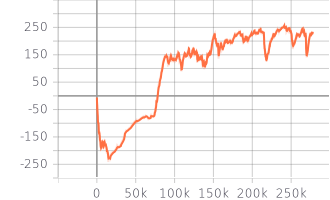
\includegraphics[width=10cm]{dqn.png}
        \caption{dqn step-reward plot}
    \end{center}
\end{figure}
\subsection{A tensorboard plot shows episode rewards of at least 800 training episodes in LunarLanderContinuous-v2}
\begin{figure}[!ht]
    \begin{center}
        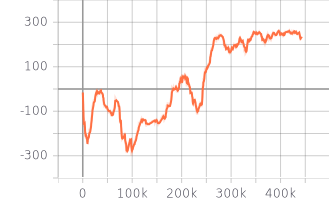
\includegraphics[width=10cm]{ddpg.png}
        \caption{ddpg step-reward plot}
    \end{center}
\end{figure}
\subsection{Describe your major implementation of both algorithms in detail.}
\subsubsection{dqn}
\paragraph{}
使用兩個相同架構的網路, 持續更新其中一個, 另外一個鎂隔一段時間才更新。網路結構如下。
\begin{lstlisting}
Net( 
  (fc1): Linear(in_features=8, out_features=512, bias=True)
  (relu): ReLU()
  (fc2): Linear(in_features=512, out_features=512, bias=True)
  (relu): ReLU()
  (fc3): Linear(in_features=512, out_features=512, bias=True) 
  (relu): ReLU()
  (fc4): Linear(in_features=512, out_features=512, bias=True)
  (relu): ReLU()
  (fc5): Linear(in_features=512, out_features=4, bias=True)
)
\end{lstlisting}
\paragraph{}
在action的選擇上, 有0.99的機率會選擇當前判斷的最優選擇(透過Q值判斷), 0.01的機率會隨機選擇action。
\begin{lstlisting}
def select_action(self, state, epsilon, action_space):
    '''epsilon-greedy based on behavior network'''
    ## TODO ##
    if np.random.random() > epsilon:
        state = torch.Tensor(state).to(self.device).view(1, -1)
        self._behavior_net.eval()
        with torch.no_grad():
            self._behavior_net.eval()
            action = self._behavior_net.forward(state).argmax().item()
    else:
        action = action_space.sample()
    return action
    ## raise NotImplementedError
\end{lstlisting}
\paragraph{}
更新參數的部份, 會先從memory buffer中sample一些記憶出來, 並且按照公式寫出q\_eval和e\_target, 這兩個數值要取mean square error, 其中算q\_target的時候不能計算gradient。其中要注意q\_eval要取出來的數值是取對應的action的數值。
\begin{lstlisting}
def _update_behavior_network(self, gamma):
    state, action, reward, next_state, done = self._memory.sample(
    self.batch_size, self.device)

    ## TODO ##
    self._behavior_net.train()
    q_eval = self._behavior_net.forward(state).gather(1, action.long())

    with torch.no_grad():
        self._target_net.eval()
        q_target = reward + (1 - done) * gamma * self._target_net.forward(next_state).max(dim=1)[0].view(-1, 1)

    criterion = nn.MSELoss()
    loss = criterion(q_eval, q_target)
    ## raise NotImplementedError

    # optimize
    self._optimizer.zero_grad()
    loss.backward()
    nn.utils.clip_grad_norm_(self._behavior_net.parameters(), 1)
    self._optimizer.step()
\end{lstlisting}
\paragraph{}
target\_network的更新方式就是每隔一段時間直接將behavior\_net的參數複製過去。
\begin{lstlisting}
def _update_target_network(self):
    '''update target network by copying from behavior network'''
    ## TODO ##
    self._target_net.load_state_dict(self._behavior_net.state_dict())
    ## raise NotImplementedError
\end{lstlisting}
\subsubsection{ddpg}
\paragraph{}
ddpg需要兩個network, 一個是actor負責決定下一步的動作, 另外一個是critic, 負責對actor做出的動作來打分數。這兩個network分別也需要各一個target network, 因此總共需要4個network。其中actor和critic的結構如下。
\begin{lstlisting}
actor
Net( 
  (fc1): Linear(in_features=8, out_features=512, bias=True)
  (relu): ReLU()
  (fc2): Linear(in_features=512, out_features=512, bias=True)
  (relu): ReLU()
  (fc3): Linear(in_features=512, out_features=512, bias=True) 
  (relu): ReLU()
  (fc4): Linear(in_features=512, out_features=512, bias=True)
  (relu): ReLU()
  (fc5): Linear(in_features=512, out_features=2, bias=True)
)
critic
Net( 
  (fc1): Linear(in_features=10, out_features=512, bias=True)
  (relu): ReLU()
  (fc2): Linear(in_features=512, out_features=512, bias=True)
  (relu): ReLU()
  (fc3): Linear(in_features=512, out_features=512, bias=True) 
  (relu): ReLU()
  (fc4): Linear(in_features=512, out_features=512, bias=True)
  (relu): ReLU()
  (fc5): Linear(in_features=512, out_features=1, bias=True)
  (tanh): tanh()
)
\end{lstlisting}
\paragraph{}
選擇action則是給定一個state, 丟進去actor network輸出兩個float, 如果是train階段擇加上一個noise達成epsilon greedy。
\begin{lstlisting}
def select_action(self, state, noise=True):
    '''based on the behavior (actor) network and exploration noise'''
    ## TODO ##
    state = torch.from_numpy(state).float().to(self.device)

    with torch.no_grad():
        action = self._actor_net(state).cpu().numpy()

    if noise:
       action += self._action_noise.sample()

    return action
    ## raise NotImplementedError
\end{lstlisting}
\paragraph{}
更新behavior network的部份, 首先先更新critic, 按照公式算出q\_eval和e\_target, 其中算q\_target的時候不能算gradient。而actor則是要希望critic輸出的值愈高愈好, 因此要最大化critic出來的值。
\begin{lstlisting}
def _update_behavior_network(self, gamma):
    actor_net, critic_net, target_actor_net, target_critic_net = self._actor_net, self._critic_net, self._target_actor_net, self._target_critic_net
    actor_opt, critic_opt = self._actor_opt, self._critic_opt

    # sample a minibatch of transitions
    state, action, reward, next_state, done = self._memory.sample(
        self.batch_size, self.device)

    ## update critic ##
    # critic loss
    ## TODO ##
    with torch.no_grad():
        action_next = target_actor_net.forward(next_state)
        q_target = reward + (1 - done) * gamma * target_critic_net.forward(next_state, action_next)

    q_eval = critic_net.forward(state, action)

    criterion = nn.MSELoss()
    critic_loss = criterion(q_eval, q_target)
    ## raise NotImplementedError
    # optimize critic
    actor_net.zero_grad()
    critic_net.zero_grad()
    critic_loss.backward()
    critic_opt.step()

    ## update actor ##
    # actor loss
    ## TODO ##
    action = actor_net.forward(state)
    actor_loss = -critic_net.forward(state, action).mean()
    ## raise NotImplementedError
    # optimize actor
    actor_net.zero_grad()
    critic_net.zero_grad()
    actor_loss.backward()
    actor_opt.step()
\end{lstlisting}
\paragraph{}
最後是target network的更新方式, 這邊採用soft update的方式, 相較於dqn的直接複製, target network會用比較緩慢的方式來更新參數, 讓behavior有穩定的target可以收斂之外, target network也可以變動的比較緩和。更新的方式就是target network和behavior network做差值。
\begin{lstlisting}
def _update_target_network(target_net, net, tau):
    '''update target network by _soft_ copying from behavior network'''
    for target, behavior in zip(target_net.parameters(), net.parameters(
)):
        ## TODO ##
        target.data.copy_(tau * behavior.data + (1 - tau) * target.data)
        ## raise NotImplementedError
\end{lstlisting}
\subsection{Describe differences between your implementation and algorithms.}
\paragraph{}
大致上來說, 實作和演算法沒有太大的差異, 唯一比較不同的就是dqn和ddpg都有對得到的reward的值域縮小, 還有dqn在更新網路參數的時候有對gradient做clipping。
\subsection{Describe your implementation and the gradient of actor updating.}
\paragraph{}
actor要儘量讓critic輸出的數值越大越好, 因此gradient直接就是critic的數值並且最大化他(加個負號變最小化)。
\subsection{Describe your implementation and the gradient of critic updating.}
\paragraph{}
critic則是要判斷某個action在某個state下的好壞, 因此要考慮到該state做這個action之後得到的reward, 以及下個state的好壞。
\subsection{Explain effects of the discount factor.}
\paragraph{}
discount factor可以決定當前選擇action時的遠見有多遠, 如果愈接近1, 代表後面的情況就會愈重要, 反之如果用靠近0, 代表愈靠近現在的狀態愈重要。
\subsection{Explain benefits of epsilon-greedy in comparison to greedy action selection.}
\paragraph{}
epsilon greedy有一定的機率隨機選擇action, 目的就是可以讓agent多多嘗試一些他現在可能判斷是不好的狀態但其實是更好的狀態, 也就是跳出現在的local minimum, 讓agent可以走到global minimum。
\subsection{Explain the necessity of the target network.}
\paragraph{}
如果沒有target network而直接用behavior更新, network的更新就很像在追著自己的尾巴跑一樣, 很難收斂。因此如果可以先固定一個學習點, 也就是固定一個target network的參數, 等到學得差不多再繼續前往下一個學習點, 因此可以讓network收斂較好。
\subsection{Explain the effect of replay buffer size in case of too large or too small.}
\paragraph{}
如果replay buffer size太小, 就很像一個人的腦容量太小, 會忘記掉過去一些還沒學到但是重要的記憶。而相反的, 如果replay buffer size太大, 會讓過去很多學習過的記憶堆積在那裡而倒置學習新的記憶的機率降低,也會對於network的學習產生負面的影響。
\section{Report Bonus}
\subsection{Implement and experiment on Double-DQN.}
Double-DQN和DQN差別只有在算q\_target的時候, 原本是找next\_state中最大的那個來計算, 現在改成在取在behavior network中最好的那個action。
\begin{lstlisting}
action = self._behavior_net.forward(next_state).argmax(dim=1).vi
ew(-1, 1)
q_target = reward + (1 - done) * gamma * self._target_net.forward(next_state).gather(1, action)
\end{lstlisting}
\begin{figure}[!ht]
    \begin{center}
        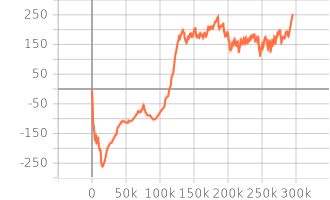
\includegraphics[width=10cm]{doubledqn.png}
        \caption{doubledqn step-reward plot}
    \end{center}
\end{figure}
\subsection{Extra hyperparameter tuning, e.g., Population Based Training.}
\paragraph{}
Population Based Training一開始產生很多個隨機參數的agent讓他們在環境玩, 挑選出那些表現比較好的, 淘汰掉比較不好的agent, 可以找到更好的hyperparameter settings而有比較好的表現。
\newpage
\section{Performance}
\subsection{[LunarLander-v2]}
\begin{figure}[!ht]
    \begin{center}
        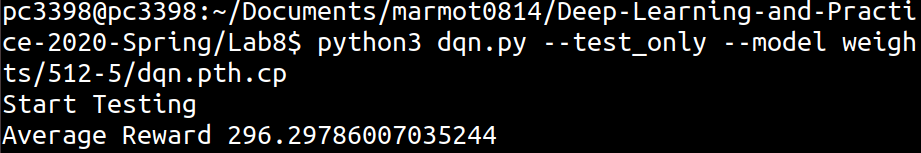
\includegraphics[width=10cm]{dqn_result.png}
        \caption{Performance}
    \end{center}
\end{figure}
\subsection{[LunarLanderContinuous-v2]}
\begin{figure}[!ht]
    \begin{center}
        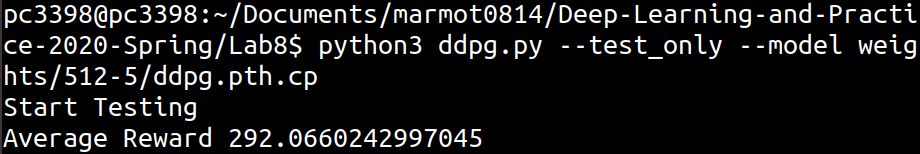
\includegraphics[width=10cm]{ddpg_result.png}
        \caption{Performance}
    \end{center}
\end{figure}
